\PassOptionsToPackage{dvipsnames}{xcolor}

\documentclass[12pt]{beamer}
\usetheme{default}
\usecolortheme{crane}

\usepackage[utf8]{inputenc}
\usepackage[T1]{fontenc}
\usepackage[slovak]{babel}

\usepackage{amsmath, amssymb}
\usepackage{hyperref, url}
\usepackage{graphicx}
\usepackage{array}
\usepackage{alltt}
\usepackage{mathtools}

%\setbeamersize{text margin left=1pt,text margin right=1pt}
\setbeamertemplate{footline}[frame number]
\beamertemplatenavigationsymbolsempty

% https://www.overleaf.com/learn/latex/Using_colours_in_LaTeX
\def\blue#1{\textcolor{Cerulean}{#1}}
\def\green#1{\textcolor{LimeGreen}{#1}}

% database-related stuff
\DeclareMathOperator{\join}{\bowtie}
\DeclareMathOperator{\antijoin}{\rhd}

\DeclareMathOperator{\lubi}{lubi}
\DeclareMathOperator{\capuje}{capuje}
\DeclareMathOperator{\navstivil}{navstivil}
\DeclareMathOperator{\vypil}{vypil}
\DeclareMathOperator{\answer}{answer}


\title{Relačná algebra}
\author{Ján Mazák}
\institute{FMFI UK Bratislava}
\date{}


\begin{document}

\frame{\titlepage}

\begin{frame}[fragile]{Relačná algebra}
\begin{itemize}
    \item interný jazyk, do ktorého sa prekladajú všetky dotazy
    \item tiež jazyk na formalizáciu relačného modelu a matematické dokazovanie
    \item zachytáva postup výpočtu dotazu pomocou\\ \alert{logických operátorov} (nezohľadňujú fyzické uloženie dát)
    \item vstupom aj výstupom operátora je relácia
    \item k danému dotazu možno zostrojiť rôzne zápisy (operátorové stromy) v relačnej algebre, databáza si sama vyberie ten, čo pokladá za najvhodnejší
\end{itemize}
\end{frame}

\begin{frame}[fragile]{Relačná algebra}
\begin{minipage}{.45\textwidth}
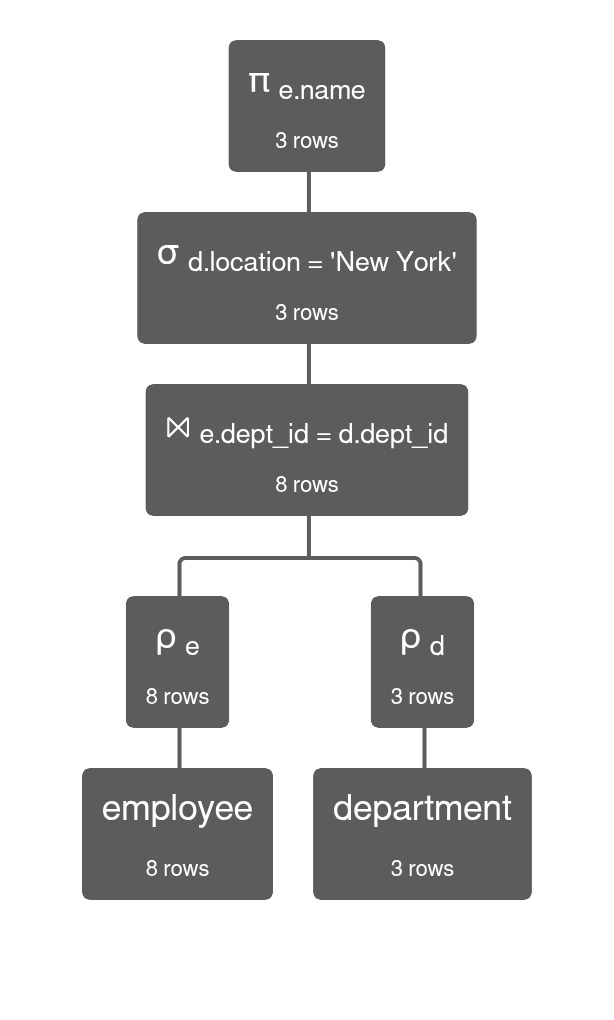
\includegraphics[scale=.2]{query3.jpg}
\end{minipage}
\begin{minipage}{.5\textwidth}
\begin{alltt}
SELECT e.name
FROM employee AS e
  JOIN department AS d
    ON e.dept_id = d.dept_id
WHERE
  d.location = 'New York';
\end{alltt}
\end{minipage}
%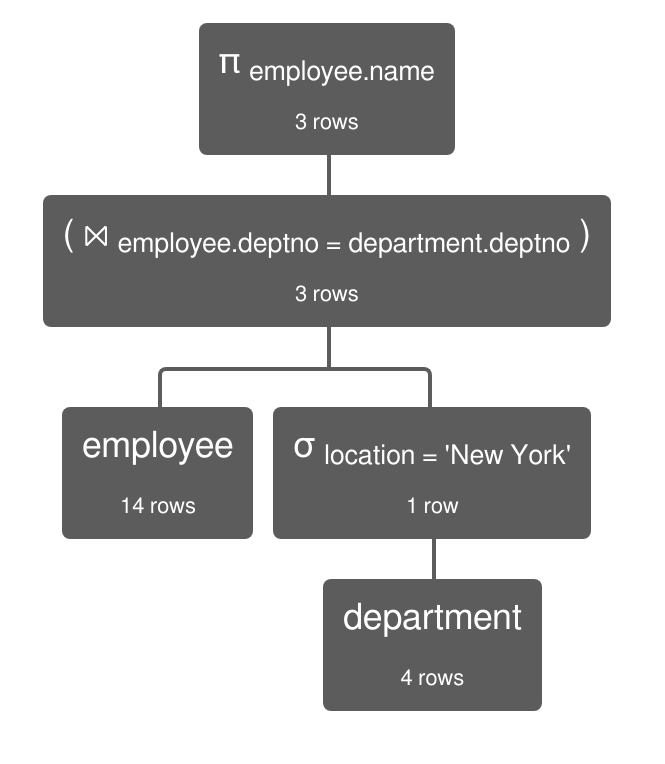
\includegraphics[scale=.2]{query2.jpg}\\[3mm]

\bigskip
\tiny{\url{https://dbis-uibk.github.io/relax/calc/gist/379b0fdd72490e8e634bb193f109d4a8}}
\end{frame}

\begin{frame}[fragile]{Relačná algebra}
Porovnajte rýchlosť výpočtu:\\
\begin{minipage}{.45\textwidth}
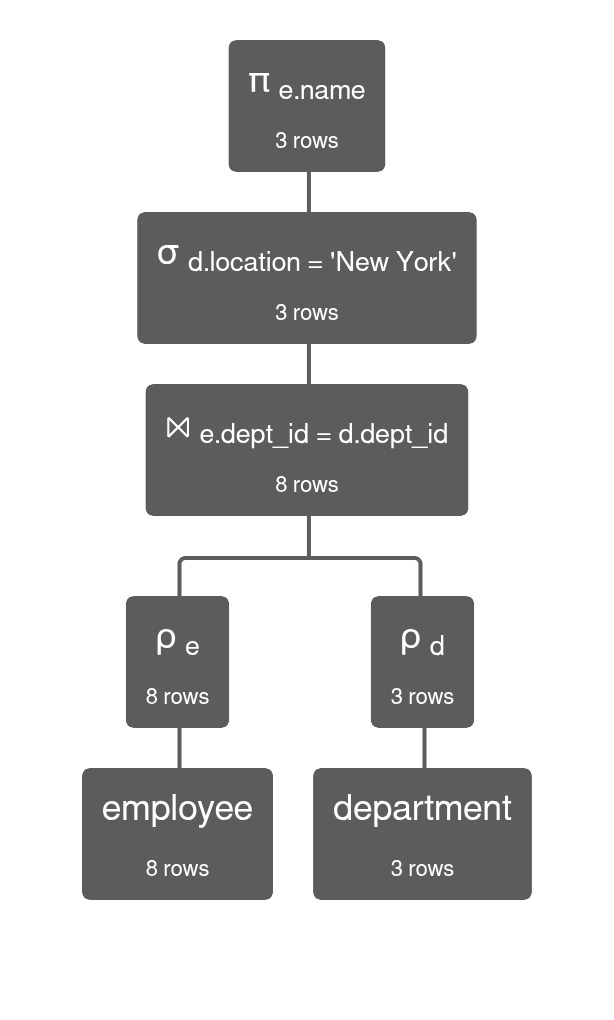
\includegraphics[scale=.18]{query3.jpg}
\end{minipage}
\begin{minipage}{.45\textwidth}
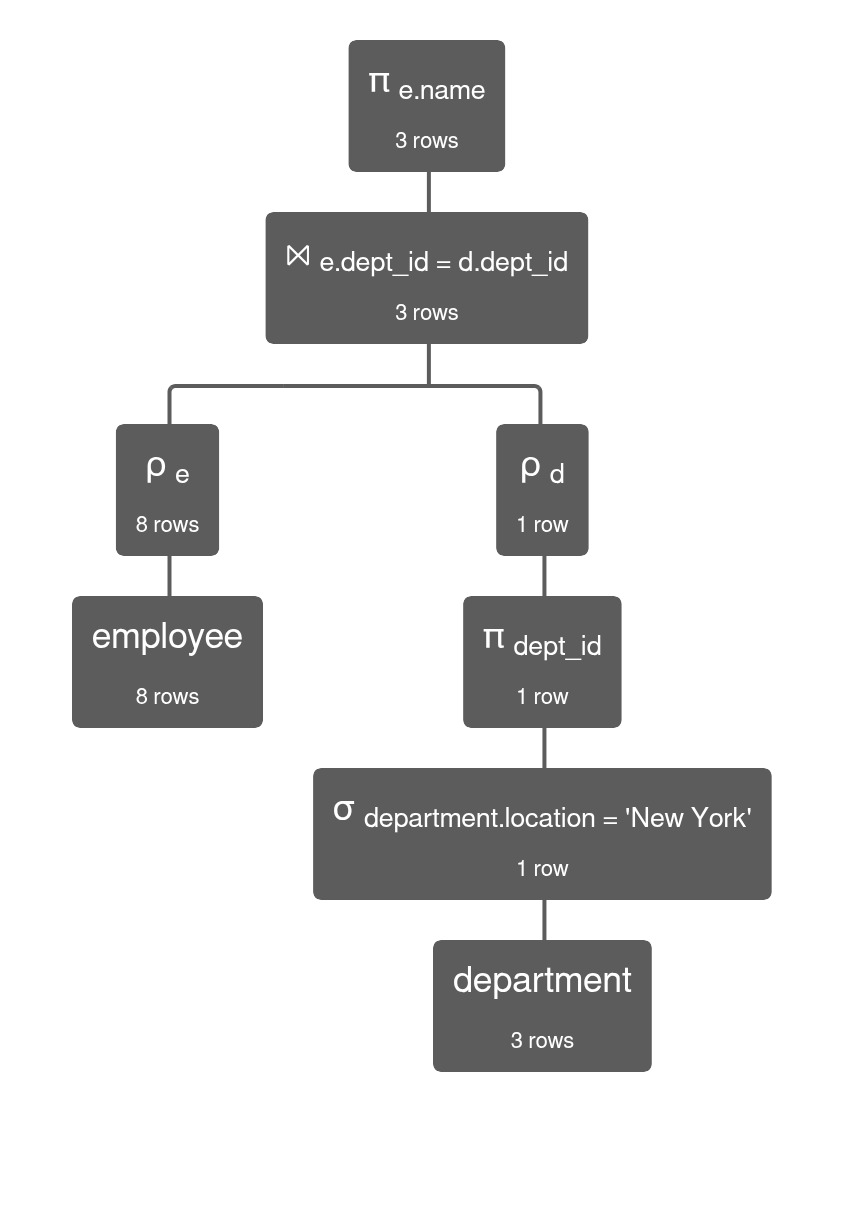
\includegraphics[scale=.18]{query4.jpg}
\end{minipage}
\end{frame}

\begin{frame}[fragile]{Relačná algebra}
\begin{minipage}{.45\textwidth}
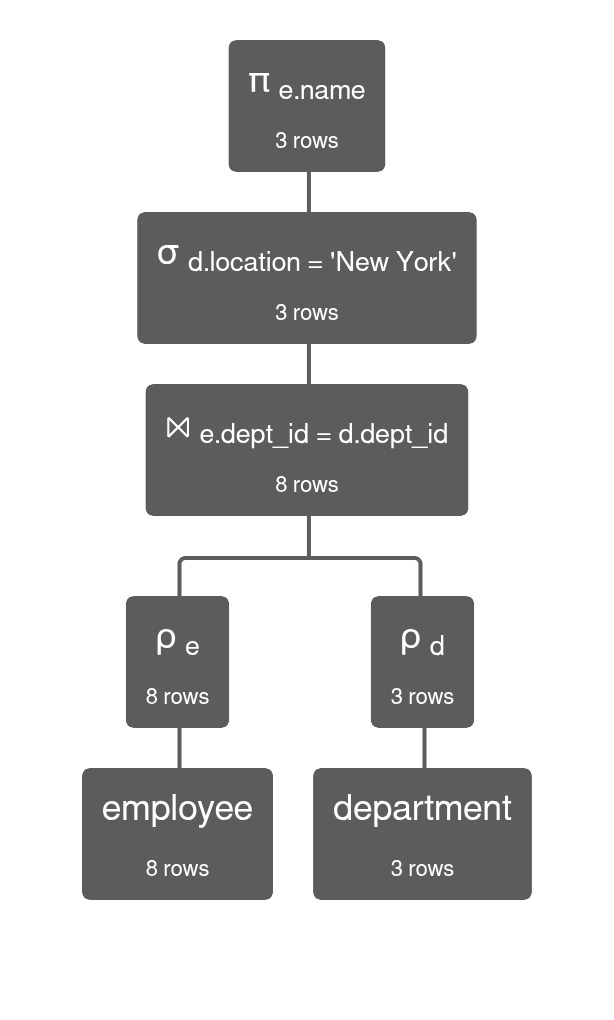
\includegraphics[scale=.18]{query3.jpg}
\end{minipage}
\begin{minipage}{.45\textwidth}
\begin{align*}
& e \coloneqq \rho_e(employee) \\
& d \coloneqq \rho_d(department) \\
& \pi_{e.name}(\sigma_{d.location = 'New York'}( \\
& \phantom{\ \ \ \ } e\bowtie_{e.dept\_id = d.dept\_id} d \\
& ))
\end{align*}
\smallskip

\begin{scriptsize}
\begin{alltt}
/* example EXPLAIN output */

Filter: (d.location = 'New York')
  -> Hash Join
     Hash Cond: (e.dept_id = d.dept_id)
     -> Seq Scan on employee e
     -> Hash
        -> Seq Scan on department d
\end{alltt}
\end{scriptsize}
\end{minipage}
\end{frame}

\begin{frame}[fragile]{Relačná algebra}
\begin{minipage}{.5\textwidth}
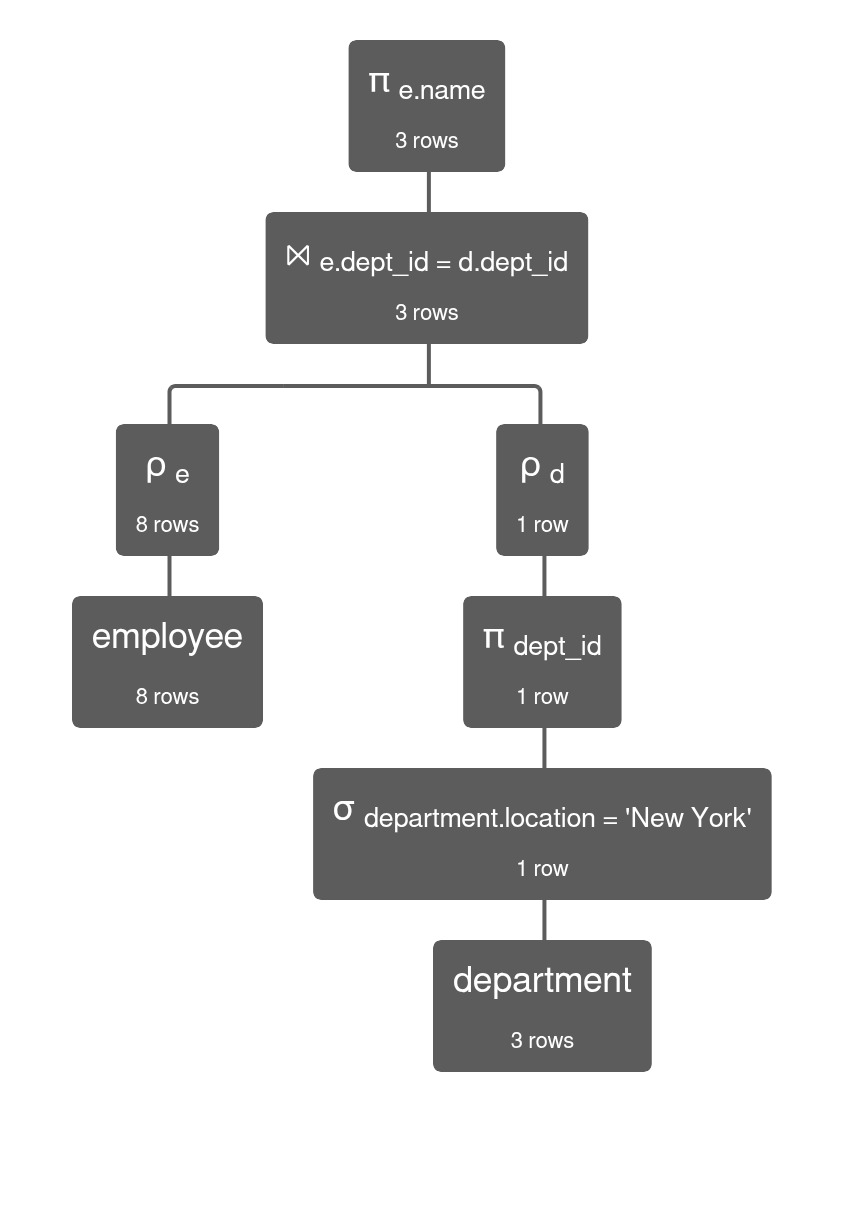
\includegraphics[scale=.18]{query4.jpg}
\end{minipage}
\begin{minipage}{.45\textwidth}
\begin{align*}
& e \coloneqq \rho_e(employee) \\
& d \coloneqq \rho_d(department) \\
& \pi_{e.name}(e \bowtie (\pi_{d.dept\_id}( \\
& \phantom{\ \ \ \ } \sigma_{d.location = 'New York'}(d) \\
& )))
\end{align*}
\smallskip

\begin{scriptsize}
\begin{alltt}
/* example EXPLAIN output */

Hash Join
  Hash Cond: (e.dept_id = d.dept_id)
  -> Seq Scan on employee e
  -> Hash
    -> Seq Scan on department d
       Filter: (location = 'New York')
\end{alltt}
\end{scriptsize}
\end{minipage}
\end{frame}

\begin{frame}[fragile]{Logické operátory}
\begin{itemize}
    \item $\pi$ --- projekcia (vyberáme stĺpce)
    \item $\sigma$ --- selekcia (vyberáme riadky)
    \item $\rho$ --- premenovanie (relácie či atribútu)
    \item $\times$ --- karteziánsky súčin
    \item $\bowtie$ --- natural join
    \item $\bowtie_\theta$ --- theta-join (join s podmienkou $\theta$)
    \item $\antijoin$ --- antijoin (riadky 1. relácie, ktoré sa nedajú joinovať\\ \hskip 2.5cm so žiadnymi riadkami 2. relácie)
    \item $-, \cup, \cap$ --- rozdiel, zjednotenie, prienik množín
    \item $\Gamma$ or $\gamma$ --- group by
\end{itemize}
\end{frame}

\begin{frame}[fragile]{Ukážky relačnej algebry}
Databáza: \emph{lubi}(Pijan, Alkohol), \emph{capuje}(Krcma, Alkohol, Cena),
\emph{navstivil}(Id, Pijan, Krcma), \emph{vypil}(Id, Alkohol, Mnozstvo)

\bigskip

1. Alkoholy, ktoré niekto ľúbi, ale nikde ich nečapujú
\blue{
$$
    \pi_{Alkohol} (\lubi) - \pi_{Alkohol}(\capuje)
$$
$$
    \pi_{\lubi.Alkohol} (\lubi\antijoin_{\lubi.Alkohol = \capuje.Alkohol} \capuje)
$$
}

2. Počet vypití piva pre jednotlivých pijanov
\green{
$$
    \Gamma_{Pijan, COUNT(Id)\rightarrow C}(\sigma_{Alkohol='pivo'}(\navstivil\join\vypil))
$$
}
\end{frame}

\begin{frame}[fragile]{Ukážky relačnej algebry}
\begin{alltt}
SELECT a1, a2, COUNT(a3) AS b
FROM r1, r2
WHERE c1 OR c2
GROUP BY g1, g2
HAVING h1 AND h2
\end{alltt}
$$
    \pi_{a_1, a_2, b}(\sigma_{h_1\land h_2}(\Gamma_{g_1, g_2, COUNT(a_3)\rightarrow b} (r_1\bowtie_{c_1 \lor c_2} r_2)))
$$
\bigskip
$$j \coloneqq r_1\bowtie_{c_1 \lor c_2} r_2$$
$$\pi_{a_1, a_2, b}(\sigma_{h_1\land h_2}(\Gamma_{g_1, g_2, COUNT(a_3)\rightarrow b} (j)))$$
\end{frame}


\begin{frame}{Literatúra}
\begin{itemize}
\item {\scriptsize\url{https://www.db-book.com/slides-dir/PDF-dir/ch2.pdf}}
\item {\scriptsize\url{https://drive.google.com/file/d/1IwVFcAWWDD_fAJAOZruXdlS3Onh3XinP/view}}
\item {\scriptsize\url{https://cs186berkeley.net/notes/note6/}}
\item {\scriptsize\url{https://dbis-uibk.github.io/relax/calc/gist/379b0fdd72490e8e634bb193f109d4a8}}
\end{itemize}
\end{frame}


\begin{frame}{Úlohy: relačná algebra}
Databáza: \emph{lubi}(Pijan, Alkohol), \emph{capuje}(Krcma, Alkohol, Cena),
\emph{navstivil}(Id, Pijan, Krcma), \emph{vypil}(Id, Alkohol, Mnozstvo)
\begin{itemize}
	\item pijani, čo ľúbia pivo
	\item koľko stojí najlacnejšie pivo?
    \item alkoholy, ktoré čapujú, ale nik ich neľúbi
    \item alkoholy, ktoré čapujú, ale nik ich nepil
	\item najdrahší čapovaný alkohol (všetky, ak ich je viac)
	\item pijani, ktorí navštívili všetky krčmy, čo niečo čapujú
    \item krčma s najväčšou celkovou tržbou
\end{itemize}
\end{frame}


\end{document}


